This chapter describes specific implementation details of the IDDR system.

\section{Overview} 
We implemented the IDDR system based on the Linux kernel, version 3.5.0 and
Xen version 4.2.1. The application domain and the driver domain run the same kernel
binary. Table~\ref{tab:base} summarizes our implementation efforts in
terms of the number of lines of code.

\begin{table}
\caption{Implementation efforts in terms of number of lines of code.}
\begin{center}
\begin{tabular}{lll}
  \hline
  \label{tab:base}
  Component & Interrupt-based IDDR & Spinning-based IDDR \\
  \hline
  Linux Kernel & 6 & 6\\
  Xen & 252 & 252\\
  Front-end Driver & 611 & 712\\
  Back-end Driver & 692 & 752\\
  \hline 
  Total & 1561 & 1722\\
  \hline
\end{tabular}
\end{center}
\end{table}

The IDDR system implementation did not require any changes to the device
driver code. However, we did make a small number of changes to the Xen
and Linux kernel.

Figure~\ref{fig:Implementation overview} shows the implementation overview of 
the spinning-based IDDR system.

\begin{figure}[!ht]
\centering
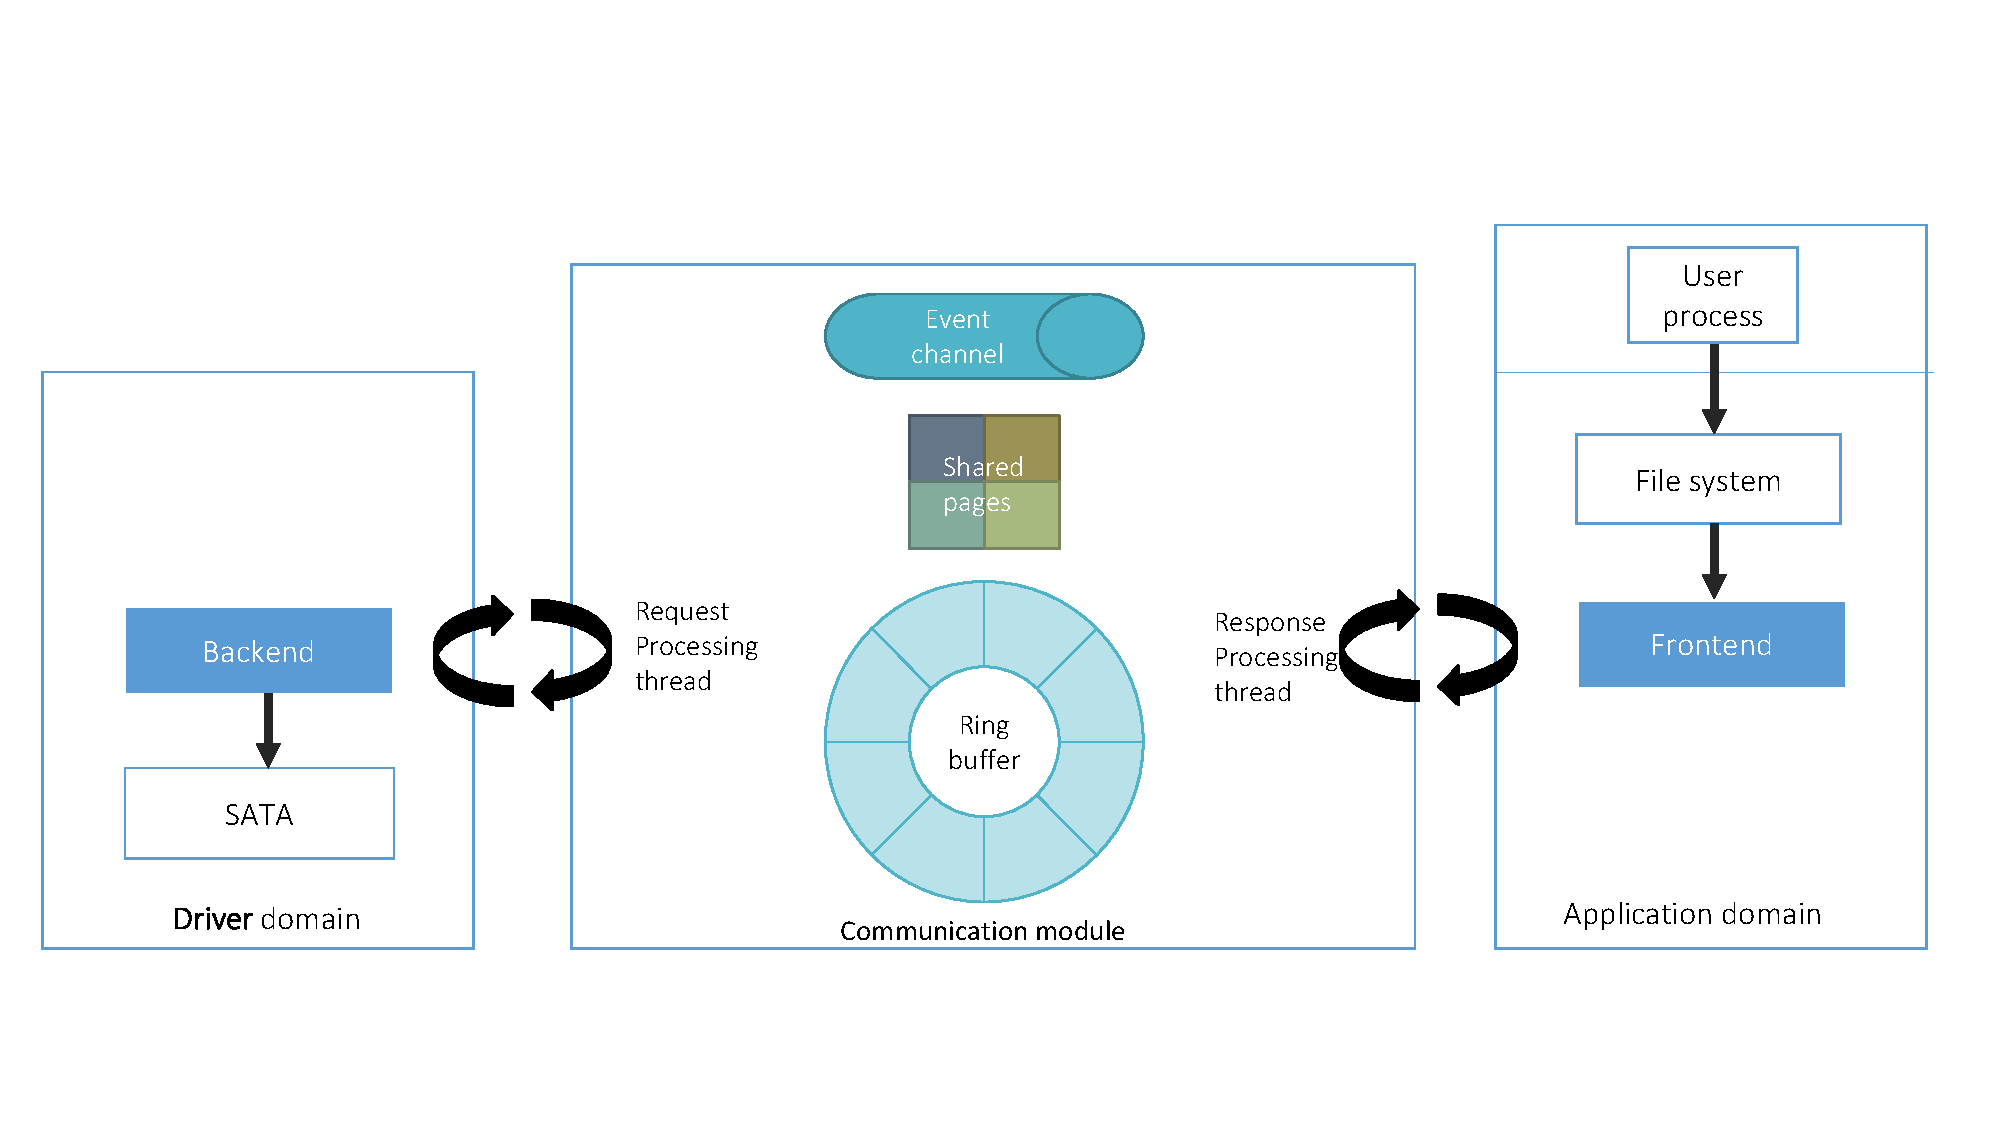
\includegraphics[width=\textwidth]{impl_overview_new}
\caption{Implementation overview of the spinning-based IDDR system}
\label{fig:Implementation overview}
\end{figure}

\section{Communication Module}
This section describes the implementation details of the communication
modules of the interrupt-based and the spinning-based IDDR systems, respectively.

\subsection{Interrupt-based IDDR system}
As Section~\ref{sub:communicationmodule} describes, the role of the communication module in the interrupt-based IDDR system is to:
\begin{enumerate} 
\item Share requests and responses between the driver and application domains
\item Share the data associated with read/write requests/responses
\item Notify the domain upon the availability of requests and responses 
\end{enumerate}
\paragraph{Shared Request and Response Queue:}
In order to implement the first role of the communication module, we
use the ring buffer mechanism provided by Xen. A ring buffer is a shared
I/O ring, which is explained in Section~\ref{subsec:io rings}. We divide
the ring buffer into the front half and the back half. The IDDR system
uses the front half as the shared request queue and the back half as
the shared response queue. 

The IDDR system allocates the ring buffer in the initialization stage
of the communication module and initializes the ring buffer in the
application domain. Whenever the frontend driver receives a request from
an application in the application domain, the frontend driver removes the
request from the device driver queue and submits it to the communication
module. The communication module checks if there is free space in the shared
request queue, and if so, allocates the space for the new
request. After batching requests together, the communication module
pushes all requests to the shared request queue.

\paragraph{Shared Memory for Read/Write Data:}
We use the ring buffer only to share the control information associated with 
requests and responses. In order to share the actual data associated with 
requests and responses we use shared pages.

As explained in Section~\ref{subsec:sharedpages}, a grant table is used
for sharing memory between domains. We use a grant table to share memory
between the application domain and the driver domain.

\paragraph{Event Notification:}
We create an event channel in the initialization stage of the
communication module in the application domain and connect to it in 
the initialization stage of the communication module
in the driver domain. We attach an interrupt handler routine for the
event channel in both domains. The interrupt handler routine in the 
application domain reads responses from the shared
response queue and forwards them to the frontend driver. The interrupt
handler routine in the driver domain reads requests from the shared
request queue and forwards them to the backend driver.

\subsection{Spinning-Based IDDR System}
This section describes the communication module of the spinning-based IDDR system:

\subsubsection*{Read response thread in the application domain:} 
In the spinning-based IDDR system we create a kernel thread called the \textit{read
response thread} during the initialization stage of the application domain's 
communication module. The read response thread spins
to check if responses are available in the shared response queue. If a
response is available, it reads the response from the shared response
queue.  If a response is not available in the shared response
queue, the thread goes into a sleep state after spinning for a set threshold duration. 
We maintain the status of the thread as \texttt{SLEEPING} or \texttt{RUNNING}
in a data structure shared between the domains for this purpose. 
When the thread exceeds the spinning threshold, we change
its state from \texttt{RUNNING} to \texttt{SLEEPING}, and we check again the
response queue for new responses in order to avoid a race condition.

A thread must not sleep unless it is assured that it will eventually be woken up.
The code doing the waking up must also be able to 
identify the thread to be woken up.  We use Linux's standard \texttt{wait queue} mechanism
to implement thread wakeup in a reliable and race condition free manner.
A wait queue is a list of threads waiting for a specific event~\cite{Galvin, Bovet:2005:ULK:1077084}. 

We initialize a wait queue for the read response thread during the initialization stage 
of the application domain's communication module. The read response thread sleeps 
in the wait queue, waiting for a flag denoting the availability of the response to be set. 
The driver domain's communication module checks the status of the read response 
thread after pushing responses on the shared response queue. If the status is 
\texttt{SLEEPING} then it sends a virtual interrupt. It uses an event channel to wake the read
response thread. The wakeup signal is sent in the form of an event channel notification 
from the driver domain to the application domain. 

Similar to the interrupt-based IDDR system, we create a new event channel in
the initialization stage of the communication module in the application
domain. We attach an interrupt handler routine for the event channel
in the application domain. In the interrupt handler, the communication
module wakes up the read response thread if it is sleeping.

\subsubsection*{Read request thread in the driver domain:}
The implementation of the read request thread is similar to
the implementation of the read response thread, except that the read request thread
spins in the driver domain waiting for requests to become available 
in the request queue.

\section{Frontend Driver Implementation}

\subsubsection*{Interrupt-based IDDR System}
The core responsibility of the frontend driver in the interrupt-based IDDR system is to:
\begin{enumerate}
\item Provide an interface which appears as a block device to file systems and user applications.
\item Accept a request from a file system or a user application
\item Send the request to the driver domain
\item Send a completion notification to a user application after reading the response
\end{enumerate}

The implementation of the frontend driver is split into 3 parts: 
\begin{enumerate}
\item Initialization code
\item Submitting requests to the communication module
\item Sending completion notifications to user applications
\end{enumerate}

\paragraph{Initialization Code:}
During the initialization phase, the frontend driver creates a separate
interface for each block device. The interface for each block device is
associated with a device driver queue. Read and write requests issued
on the interface are queued in this device driver queue.

\paragraph{Request Submission:}
The frontend driver removes the request submitted to the driver
interface and converts the request into a request structure, which is
required by the backend driver. The request structure points to
the shared memory allocated for the read/write data by the communication
module. The frontend driver then forwards the newly created request
to the communication module, which submits the request to the
backend driver.

\paragraph{Completion Notifications:}
We maintain a shadow table that contains an entry for each request that was 
received in the device driver queue. 
We implement the shadow table as a circular
array whose entries refer to these requests. We maintain an ID for each request. The backend
driver copies this ID into the corresponding response. The ID is used
for mapping the response to the request in the shadow table. When a
response is read by the communication module, it forwards the response
to the frontend driver. The frontend driver looks up the corresponding
request in the shadow table, and sends a completion notification to 
the user application that issued the request.

\subsubsection*{Spinning-Based IDDR System}
The core responsibility and implementation of the frontend driver of 
the spinning-based IDDR system is similar to the frontend driver of the
interrupt-based IDDR system.

\section{Backend Driver Implementation}

The role of the backend driver in the IDDR system is to:
\begin{enumerate}
\item Read a request through the communication module and convert it to a block I/O request
\item Accept a response from the block device driver
\item Forward the response to the communication module
\end{enumerate}

The implementation of the backend driver is split into 2 parts. 
\begin{enumerate}
\item Forwarding requests to the actual block device in the required block I/O request format. 
\item Forwarding responses to front-end driver.
\end{enumerate}

\subsubsection*{Request Forwarding}
\label{subsec:createbio}
The backend driver converts a request that is received via the
communication module into the required block I/O request format (using \texttt{struct bio} objects
as discussed in Section~\ref{subsec:request queue}), so that the block device
can process the request. In order to create a block I/O request, pages from
the shared memory are mapped and inserted into the block I/O request structure and
any required information is copied from the shared request into the block I/O
structure. The newly created request is sent to the actual driver execution. 
Once the block I/O request's execution is completed, the driver calls a provided
callback function.

\subsubsection*{Response Forwarding}
Irrespective of the success or failure of a request's execution,
the backend driver forwards the real device driver's response to the frontend
driver.  The result of the execution and a request ID are
copied into a newly allocated response structure. The request ID is used
as an index in the shadow table to map responses to requests. The
communication module pushes the response into the shared response queue, 
so that the response is made available to the application domain.

\subsection{Future Work}
\paragraph{Adaptive spinning: }
In the current implementation the read request and read response
spinning thresholds are set to be constant amounts of time. 
As future work, adaptive spinning could be implemented in which the
threshold is varied based on assumptions about the cost of blocking
and resuming the respective threads.

